\Chapter{Men and Their Monuments}{Glyn Court}

Most of our wood carvings, it must be admitted, have no strange, eventful history, but they do represent an art which has not altogether lost its following, and they also serve me to introduce the character of my Uncle Lewis, who, like his brother William, practised wood carving with enthusiasm and considerable success; moreover, he loved the old life of our valley and committed to writing innumerable memories which else would have been lost beyond recall.

Lewis Henry, the eldest child of William, was born in Roadwater in 1870, at the same hour of the same day as his grandfather George, fifty-five years before, and he received the education that the parish had to offer: two year's at a dame school near the Valiant Soldier, two at the Church of England school in Leighland, and two more, when High Church influences were making grandfather uneasy, at the Wesleyan Day School in Washford. By then the closure of the mines, the flagging condition of agriculture, and grandfather's support of the Good Templar movement had so gravely injured his business that, with heavy heart, he had to take Lewis away from school at the age of twelve and a half, and the boy worked at the bench until there came an opening in the post office, and life began to broaden out. As a postman he was earning fourteen shillings a week - three or four shillings more than a labourer with a family to support ~ and his delivery round took him on foot over much of the Brendon Hills, covering fifteen or sixteen miles a day. At the furthest point of his travels he would have a wait of three and a half hours in an old railway hut, and he passed this time to advantage by buying a few books, including a Latin grammar, and studying them assiduously to improve his knowledge of literature and the world.

From his early years he had been unusually sensitive to the beauty of Nature, and when, at the age of ten, he with a number of other boys experienced conversion in a revival meeting, in a moment every feature of the landscape became, for him, transfigured; as for Wordsworth, each object, the stream, the hedgerows, the apple blossom, became \quotemark{apparelled in celestial light}. At sixteen he became a preacher and was eventually recommended, very much against his will, for the Bible Christian ministry. He went off to Portsmouth to preach his trial sermon, hoping and hoping that he would be rejected. To no avail: he was accepted, and began a remarkable career.

He was first sent to the Isles of Scilly, where the attention of the warmhearted Islanders softened the inevitable pangs of homesickness; (sixty years later his hosts were still sending him flowers). The seclusion and the absence of distractions made ideal conditions for his new studies, and the sea and the boundless sky, the majesty of the storms, the rich sunsets, the luminous air, made a profound impression on him. As he sat one evening on a cliff looking out toward Bishop's Rock, he heard of the death of Tennyson, whose poetry he had learnt to love in company with his dearest friend, the young organist of Roadwater. Now, the splendours of sunset and the moaning of the waves at the foot of the cliff stirred deeps in him that he had never known, and the mysteries of life, death and eternity swept in upon him with overwhelming force. That evening opened up to him a new world of thought and emotion that was to enrich his whole life. He discovered a gift for verse, and employed it for fifty years. He had a poet's faculty of seeing the eternal and unchanging in the ephemeral and everyday, and he had inherited his father's facility in the use of words. Scenes of daily life and, perhaps most of all, memories of Somerset awakened emotions which needed to find immediate expression.
He did not strive after a painful and insincere originality, and it is not surprising that his devotion to poets of the past should sometimes have caused him to indulge too freely in the stylised poetic vocabulary of a former day. But his poetry was always genuinely himself, and it was read with affection by thousands who shared something of his experience of religion, beauty and art.

His first duty and his first pleasure was, need I say, the calling to which he had devoted himself, the exacting work of a Methodist minister, and he fulfilled it tirelessly and memorably.

After his superannuation he turned for creative relaxation to wood-carving and made oaken sideboards, overmantles, cupboards, bookshelves, but all his other work continued, preaching, visiting, writing, raising funds - he would walk ten or twelve mile a Sunday into his eighties. But inextricably linked with his devotion to his calling there had always been his love for the scenes of his childhood, for the memory of the men and women who had lived among them and given them life, and for the Bible Christian Church to which he owed his life's happiness. For all these he felt a gratitude which could only be expressed by re-creating the golden past; in pursuit of this he assembled, over half a century, an unequalled collection of letters, documents, photographs and souvenirs of his Church and wrote article after article on the characters, customs, homes and trades of our valley in the days of his youth: and I for one own the debt as incalculable.
 
\section{The Sofa}

To look at it, you would think it a very dowager of a sofa, and one of the old school, making few concessions either to elegance or to bodily comfort, A straight back, hard head-rest and horsehair seat might have delighted St Anthony, but even the resilient Victorians, you feel, might have drawn the line at such lack of comfort. But of course standards of comfort and luxury change, and privileges become prerogatives, and new generations make new demands; and the owner of this sofa in the late nineteenth century was not a fanatical ascetic but one of the gentlest souls who ever drew breath.

Like so many others in this history, Jim Slade was born in Roadwater, in the short period of prosperity coinciding with the working of the iron ore mines on Brendon Hill. His father Thomas, a blacksmith, had a modest share in this prosperity, for he was a hard worker and skilful, but the real business of his life was conducted outside the forge. He was wholly untainted by personal ambition, and his great care, after his family, was the village chapel, where he led the orchestra with his bass viol, and to whose progress he greatly contributed in later days. James inherited little of his father's strength, but a double portion of his musical skill, with his tender musician's fingers, and at eight years of age he was regularly playing the harmonium for Sunday services.

The course of his life was set plain, and his conversion while still a boy was almost a natural outcome, and one from which he never retracted. He became bound in friendship which became deep and lifelong with Lewis Court, and the two young men would share their thoughts and their hopes as they sat on summer's evenings on the wooded hillside behind the chapel and read Tennyson and Browning together. Lewis left home for the ministry, but Jim's delicate nervous constitution barred him from such a hard life of wandering. He stayed in the village and became the friend of Lewis's younger brother, Will.

He never lacked employment. His work as a music teacher occupied his days and brought him an income sufficient for his few needs, and his reputation grew; people regarded him with respect for his talent and affection for himself. To his friends he recounted a meeting on Taunton station with a Doctor of Music from Dunster, from whom he had had lessons many years before: \\


\begin{quote}
\quotemark{I don't know whether you remember me, Doctor. My name is Slade.} \\
\quotemark{Remember you? Of course I do. After all this time I don't suppose it  will do you any harm to be told that you were the aptest pupil I ever had.}
\end{quote}

His \quotemark{free} time	was taken up with training the chapel choir and from time to time organising concerts in the Temperance Hall, and his Sundays with playing	the organ and teaching in the school. Then came the Great War, and the contented, self-contained village life drew to a close. The rigours of those years told hardly on him, especially as he felt constrained to undertake duties for which he was physically and temperamentally ill-suited, as a postman on weekdays and a local preacher on Sundays. His health gave way and he suffered a nervous breakdown, and though he recovered and experienced the delight of playing the singularly sweet-toned organ installed in the new chapel, his frail constitution had reached its limit. He only lived to be fifty-three and, after an early disappointment, he had never married, but his passing, and the memory of his music, caused his dearest friends a feeling of loss to which they were never wholly reconciled and an emptiness which no new friendships could ever fill.
 
\section{The Engravings}

The readers who have borne with me thus far will, I hope, agree that it is not parochialism that prompts the claim that this little plot of earth has produced a harvest of men of character out of all proportion to its acreage. We have good cause to be proud of the labourers and landed men who fashioned our landscape, of the builders who built our cottage homes, of the teachers who gave instruction, and of the preachers who taught wisdom. Nine out of ten of our forefathers passed their lives in backbreaking toil and left no memorial but a season's furrow; it was the one in ten who gave the work of which I have just written and who, through the byways of heredity, brought out here a writer, there an engineer, here a musician, there an architect, here a scholar, there a preacher. Yet it is a remarkable fact, for which I can offer no satisfactory explanation, that no artist of high rank has gone out from among us. Lack of opportunity cannot be an adequate explanation. It was a wise Dr Johnson who wrote, \quotemark{Slow rises worth, by poverty depress'd}; but if the talent is there in sufficient strength and sufficient number, some of it will find eventually a way through. Sad to say, despite the unequalled man-made beauty of our landscape or perhaps because of it, we have not produced a landscape artist.

On the other hand, we have not been wholly neglected, and artists of international repute have visited us and even made their homes among us. The beauty of our rounded, heather-clad hills and wooded combes has given delight to the most unexpected characters, from mediaeval monks to modern machine-minders, and it is no wonder that creative artists have revelled in the harmony of colour. Turner paid us a visit on his tour of the West Country and south coast in 1821, and left a record of Watchet harbour and West Cliff, and of Blue Anchor, the Dunster marshes and the distant heights of Exmoor - and if the second picture, in Turner's inimitable way, shows a landscape re-arranged to the artist's taste, we feel there would be little point at this date in complaining to his somewhat impatient shade.

It was not until the 1870s that the railways made communication with the outside world - for what it is worth - generally practicable, but eventually a group of painters - one must use the word \quotemark{group} even though they were not formally connected - came to accept the beauty of Somerset for itself without need of rearrangement, and settled among us. They were all of considerable renown and accomplishment, and two, possibly three, of them possessed qualities of originality and characterisation which make their subsequent neglect hard to account for except in terms of aesthetic fashion.

The first of them was J. W. North, a water colourist with a most acute sense of colour, who settled at Baggearn Huish House in 1885 and became very much involved in the life of the neighbourhood. He was a vigorous, dedicated Liberal of the Radical wing, and found himself more than once involved with petty tyrants over questions of public rights. His pictures have been dispersed among various art galleries, but one in Birmingham shows a riverside scene from our valley.

The second painter was Robert Walker, a disciple of Courbet but with a more sympathetic attitude to his subjects - unless it were that the subjects were more humane. Walker came under the influence of North in his landscapes, and his \quotemark{Plough} and \quotemark{The Old Gate} were painted in the neighbourhood.

Little is known to me of Robert Macbeth, except that he came to live in Bilbrook, on the road from Washford to Minehead. Like North, he was a water colourist and greatly influenced by him. But the fourth painter was known to all the art world of the late nineteenth century and his reputation was international.

Sir Hubert von Herkomer, the son of a Bavarian wood carver came to England in 1857. He was an outstanding example of the old industrious but warm-hearted German of pre-Empire days, and moreover he was an undoubted genius whose creativity took many convincing forms. He not only established a reputation as a portraitist of great insight and a genre painter of profound social sympathy, but also produced original work as an architect, interior decorator, operatic composer, orchestrator and melodist and toward the close of his life, producer and director of his own films. He excelled in all he attempted, not least in his family life. In his late forties, however, he detected a slight falling off in his awareness of colour nuances, and in 1892 decided to move from his home in Bushey to Somerset. His expressed reason is interesting: he wished to benefit from the company of J. w.  North, whom he described as \quotemark{a great colourist and a good friend} - and North's disciple Robert Walker had been Herkomer's early idol and examplar. But even more interesting are his mixed reactions to what he found:

\quotemark{The house was un-get-at-able, and the loneliness at first appalling!} Country life was more primitive than he had bargained for, and he was suffering abdominal pains which made work a severe trial of his fortitude; \quotemark{but} he cried:

\begin{quote}
\quotemark{what a country for the artist! 	 The rich red soil, the undulating country, the apple trees tumbling about in their eccentric untouched shapes ... the dilapidated farmhouses; all a treasure ground for painter and poet. In spring, the first budding of leafage, like jewels set in the deep purple tonality given by the massing of tree branches not yet inleaf, the offset of the strong green masses of ivy growths that have taken overwhelming possession of the stems to which they are attached, give a witchery to this corner of England unsurpassed, \\
I should say, in any part of the world,} \\
We should only demur at \quotemark{I should say}.
\end{quote}


\section{The Boneshaker}

How anyone can have contrived to propel our \quotemark{penny farthing} along the rutted Somerset lanes of the 1880s passes my understanding, but propel it they did, probably by placing both wheels in the same rut, leaping aboard, and pedalling for dear life.

The acknowledged master pedaller was John Bond, and there is quite a story attached to his name. 

He was born in December 1850, the eldest son of Willliam Bond, a herbalist. Round about his eleventh or twelfth year, I suppose, he was apprenticed to one of the Roadwater blacksmiths and towards the end of his apprenticeship - possibly for his master-piece - he decided to make a penny farthing. These machines had been made commercially for some time past and manufacturers were evolving lighter and more elegant models. But in general they were for gentlemen of leisure or the new well-paid urban middle class, not for the penurious countryman. John Bond's machine was the product of our simpler rural society; the essential bicycle, able to endure hardness, and offering no concessions to the weak.

\begin{figure}[!b]
     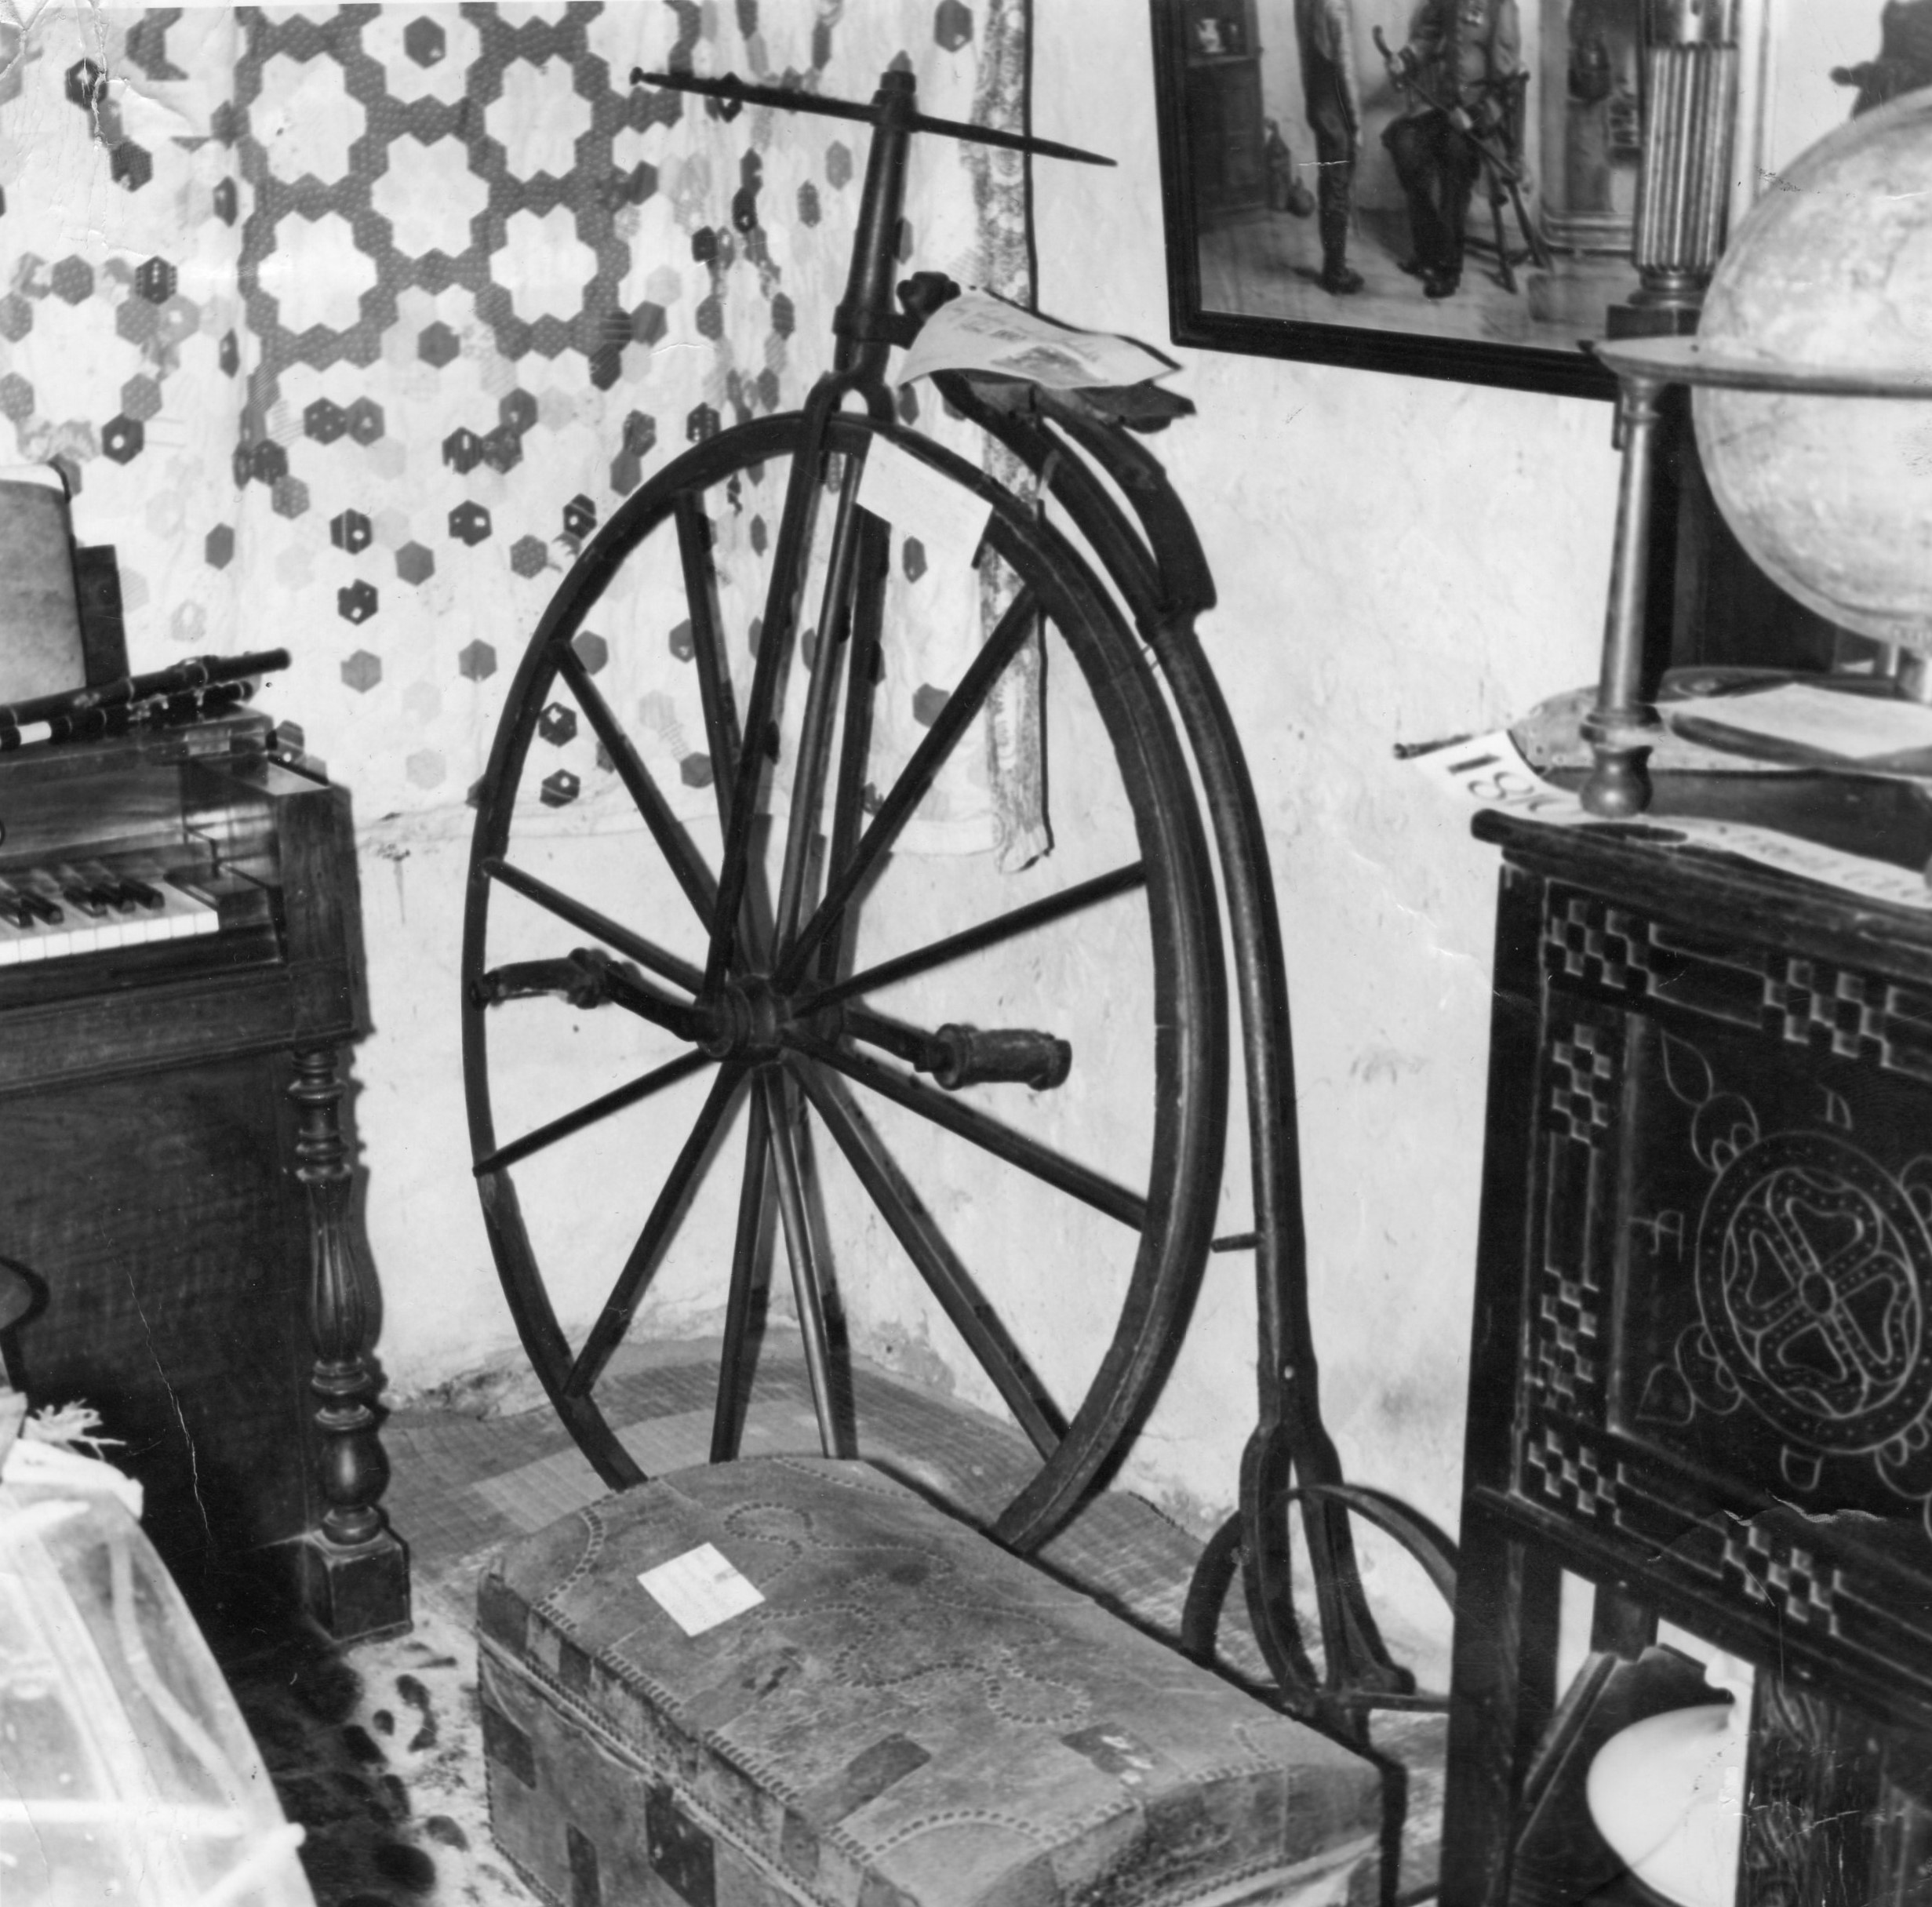
\includegraphics[width=1\textwidth]{figures/Boneshaker}
     \caption{The Boneshaker, the penny farthing used by John Bond, on display within the Museum. The bike can still be found to this day within Roadwater Village Hall.}
     \label{fig:SomersetLife}
\end{figure}

The front wheel is of moderate height and the hub, the wooden spokes and the felloes are the work of a craftsman - probably the village wheelwright, Thomas Popham - but they are enclosed by an iron tyre half an inch thick, shrunk on to the wheel. The front forks are of hammered iron, and their shaft passes through the straight handlebar and is secured by a heavy bolt. The frame is a tubular S-bar with a projecting horn for the saddle and a simple upping-step. The twelve-inch rear wheel is more sophisticated, bound with a shaped rim which once carried a tyre, but the whole machine is of a massive simplicity. Even the saddle was an iron sheet, though no doubt it originally had a leathern cover.

John Bond took up his father's trade and travelled far and wide in Somerset and Devon suitably dressed in top hat and frock coat, and administering his herbal medicines to men and beast - the same medicines - with equal success. His penny farthing, of course, he only used locally, but his boys kept the wheels turning merrily and it remained much more than a nine-day wonder. John's nephew told me:

I can mind father telling me about a time they were up \quotemark{Mount Lane} (a steep hill in Roadwater with a hairpin bend);

\begin{quote}
 \quotemark{There were three of them up - Father on the seat, another boy on the step and another one sat on the handlebar playing a concertina. They came down the hill fine and picked up speed; but it was a rough old lane in those days and at the bottom the front wheel hit on a great stone. 'Twas a good job there was a hedge, because they all three of 'em got off a lot faster than they got on.}
\end{quote}
 
 
After twenty or thirty years of use the penny farthing was superseded by one of the new factory-made safety bicycles which, perhaps more than any other single factor, changed village life and destroyed the old self-contained society. The machine was left in an outhouse, until my father retrieved it as a memento of happier days. Years later, finding that he no longer had room, he deposited it on loan to Taunton Museum; and thence, forty years on, the penny farthing, by a natural movement, again found itself in the parish where it had been made.
 
\section{The Post Office Clock}

This clock may well be unique, unless a few remain in post office museums. The hours are marked by the letters A to K instead of 1 to 12, and the minutes between the hour markings by STUV. The clock was used in the old Washford Post Office in Victorian and Edwardian days, when telegrams were sent by Morse code, with the aid of a buzzer which gave two distinct tones, high pitched for a dot, low for a dash. The system of dots and dashes for numbers had not yet been devised, and times in the text of a telegram were given by these letters. Thus a telegram might read Arriving Washford 10.33 - and would be sent as Arriving WCR JFU. From TU (Taunton) to WCR (Washford).

My mother who came to the post office as a girl in 1902, rapidly became the most proficient telegraphist in the district.
 
\section{The Motor Cycle}

Like many another relic, the motor cycle stood unattended in a shed for forty years. Yet it was a splendid machine, a 600 c.c. chain-drive James which first saw the light of day in 1914. My father bought it, complete with a plywood sidecar, about that time (or maybe after the war) for £65, which was no small sum.

The original instruction book is still with us. The powerful machine needed to be treated with respect, and Father liked to tell us that the first time he tried to ride the James, she threw him off. Still, there was space to learn for the roads were unencumbered; and right up to his dying day he found it hard to accept that other motorists might, from time to time, be using the same stretch of road as ourselves. Providence, of course, worked hard on his behalf, and only once did he come close to an accident, when the James took the bit between her teeth in Carhampton, charged up behind an old woman of the village who was fetching water from the pump, and sent her buckets flying all over the road. My father knew better than to wait for explanation, nor did he linger in Carhampton on his way home. 

He and my mother went on their honeymoon in the James, and they recalled that the hundred miles from Washford to the Wesleyan Chapel in Swindon, where they were married, had taken only a gallon and a pint of petrol. He went on using the combination till about 1928, transporting his stock to and from Roadwater, in the sidecar, with his son perched on the top and gazing for the lights of home on thehillside as they came down the valley. Then he bought a motor car, an open Calcott I tourer, for £450, and within a couple of years the road tax went from ten shillings to as many pounds, and the Calcott languished in the garage, gathering dust, until he sold her in the early 1930s to a scrap dealer - to my boylike regret, even then - for £2.
 
\section{The Band Books}

Three much-used oblong quarto music manuscript books, two of them in homemade bindings of pigskin, but all filled from cover to cover with compositions for wind band, all the parts neatly written out in brown ink, and bearing such an unexpected assortment of titles as \quotemark{Queen Victoria's March}, \quotemark{The Somerset Waltz}, \quotemark{With my pipe in one hand and my jug in the other} and \quotemark{Awake, arise, with angels sing}, and inside the front covers \quotemark{This book belongs to George Matthews, Pitt Mill, 1838}: these are a simple record of much activity.

Millers, in the old rural society, were not always the most popular of men, particularly on the manorial estate; they were suspected of every kind of sharp practice from the exercise of monopoly to the adulteration of the flour they ground. But no such suspicions attached to George Matthews. He plied an honest trade and devoted his leisure hours to the music of the church, in the hamlet of Leighland on the hillside above his home, and the little church orchestra, as the Union Band, doubled the role of village band for the revels and other rare festivities which broke the harsh monotony of the farm labourers’ round. Probably the band was heard to better effect in the open air than in the church, for the instruments as noted in the band books were, one might say, competitive in tone: two clarionets, an octave clarionet, a cornopean or two-valved cornet or a bugle, two B flat horns, a trombone and a \quotemark{sarpent}. In the matter of blending they would have left much to be desired, but George Matthews made the best of his resources, and at the close of the day he would often sit by the light of a candle and \quotemark{prick in the notes} of an arrangement of a popular air or hymn tune or, more often still, compose carols, dances and marches which were within the compass of his players. Whether he had received any musical training I do not know; from the occasional inadequacy in his harmony I suspect that he had not, and the neatness of his notation marks him as an amateur! But that was of no consequence. He was an enthusiast, a creative musician, and also a disciplinarian who imposed his will on his bandsmen so that they performed better than they had thought possible.

George's method of rehearsal was individual. His mill stood by a stream in a deep valley of green fields and winding lanes. He would assemble his bandsmen in a field above the mill, run over a piece with them, issue his instructions and then withdrew to the opposite side of the valley and conduct from there. If all went well he would radiate contentment. But woe betide the musician who played a wrong note! George would come coursing down the hillside, across the bottom and up to the offending bandsman, and upbraid him with such energy that the rest of the performance was flawless - unless, of course, the poor fellow was so shaken that false notes henceforth flowed in a stream.

At Christmastide they kept up the fine old customs of the waits, as Hardy so lovingly depicts them in \quotemark{Under the Greenwood Tree}, but these reached their peak under the leadership of George Matthews's musical successor, Thomas Slade. Thomas, born in the early 1840s, had known a childhood of dire poverty as one of the numerous family of a roadmender, but he had been apprenticed to one of the Roadwater blacksmiths, and his skill and industry won him independence. But man of business though he was, he was much more a man of music. Except in the company of his family and friends, he was reserved, even taciturn, and music, to him, meant more than words; if a dark mood fell on him, music would charm It away. One who knew him speaks of his musician's ears and delicate, tapering fingers, apparently so unsuited to the work of a blacksmith. In him there was a hunger for beauty of sound which would only be satisfied by a mellow concord of instruments. As a youth he conceived the desire to play the \quotemark{bass viol}, as the 'cello was called, so early one morning he took some of his savings, walked the twenty miles to Taunton, purchased the \quotemark{bass viol}, brought it home another twenty miles on his back, and did two hours' work in the forge before retiring to rest. He soon became a proficient player - not a virtuoso by any means, I suppose, but he held his line as choirmaster and leader of the orchestra of the village chapel with singular sweetness of tone. Local lore treasures the tale of one incident which took place in one village church:

Parson: The choir and orchestra will now render an anthem: Who is the King of Glory?
Bass violist (sotto voce): Pass the rozzrum, Bill, us'll show en who’s the king o’ glory!

I wish I could attribute it to Thomas, but it does not seem quite in his character. Yet he had his festive side, and more even than the music of the Sunday services he loved the festival of Christmas. Both spiritually and musically it crowned his year, and the old carols which George Matthews had made popular were his delight as well, with their dignified phraseology, foursquare melodies and energetic fugal choruses: Angels from the realms of glory; Behold, what glorious news is come!; Mortals awake, rejoice and sing! He spared no effort to make the performance worthy of the occasion. The band and singers would meet for rehearsal in the week before Christmas, and late on Christmas Eve, when most of the village was asleep, they would gather with their instruments in the forge, threading their way by the glow of the embers past coulters and ploughshares and every kind of farming implement, and assemble in Thomas's parlour for hot peppermint cordial to fortify them for their journeyings. Then they would set off on their round of the outlying farms where they knew they would be welcomed. Excitement and laughter were in the tingling air, but as they drew near to the first farm, they all fell silent at Thomas's bidding. To his mind, music was the sister of silence; there must be no disturbance of the quiet of the night; the sleepers should be wakened not by a babble of inconsequential noises but by a concord of sweet sounds. The band would strike up the major chord which gave the singers the key, and presently a light would shine in an upstairs room, a window would open and a voice call out a greeting, then the front door would open and the waits would troop in to taste the refreshments laid out for them; then on to the next farm, and the next until at two o'clock, some of them steadier on their feet than others, they found themselves back on the bridge that formed the centre of the village, giving their retiring serenade to an appreciative, if somnolent, public. One further performance at the morning service closed their Christmas oratorio for that year; the carols would continue in Thomas's home, around his son's piano, over Christmastide, and the simple festivities and the visits of friends and relations would go on until Old Christmas Day, January 6th; but nothing could induce Thomas to sing or play one of the carols out of that season; he would have considered it an affront to the divinely appointed order of things. The carols, for being performed only in their due season, were all the more prized.
 
\section{Marine Relics}

It is with embarrassment that I confess to a lack of the true-born Englishman's love of the sea. In fact, for one born almost within sight and sound of salt water, I am inordinately suspicious of the stuff. Fortunately some of my ancestors were cast in a sterner mould and led a seafaring life. Great-great-grandfather, Richard Grinslade, who flourished in the first quarter of the nineteenth century was a mariner of Watchet - not a captain, as far as I know; besides, he would have commanded a crew of two or three at most, for the boats which sailed from Watchet harbour were mostly small craft, fishing smacks and the like. They were very numerous, however, and at the height of the shipping trade some sixty craft were registered in Watchet.

Whether Richard owned one or not, there was no boat for his son George. Richard was thrice married. His first wife died after eighteen months; his second marriage, with a cheerful little soul, lasted as many years, and George was born to them on 31st October 1815. (I note, in writing these words, that it was a hundred and sixty years ago to the very day - or, as my mother would have said, \quotemark{Your great grandfather would have been a hundred and sixty if he'd lived.}) But Richard's third wife had no love for her stepson, and he was sent off while very young as apprentice to a shoemaker in Dunster.
To telescope the events of half a century, George worked hard at his craft, attained a good financial position, invested in houses - for in those days the ownership of property was thought to confer rights and a good return of investment. In 1870 he ventured on a different type of investment and bought a half share in a boat, a forty ton ketch, the Union of Watchet.

His partner was, in his own way, as remarkable a man as George himself, a young sea captain, John Short by name, from one of the best-known Watchet families and married, I believe, to George's niece. Thirty years later he took his place in history when Cecil Sharp came to West Somerset in search of the vanishing folk songs. John Short, who possessed a fine baritone voice and a prodigious memory, gave him the words and music of over forty of the old songs - a greater number, I believe, than any other singer in any county. The Oxford Companion to Music contains a picture of him seated on the steps of Watchet West Pier.

The partnership went well for a couple of years. The \quotemark{Union} was, like most of the Watchet craft, engaged mainly in the Bristol Channel trade, which gave the advantage that although the risk of shipwreck was as great as anywhere in the world, the voyages were short and the returns fairly rapid. She cost more to refit than they expected, but after that she plied steadily round the Bristol Channel and along the north coasts of Cornwall and Devon, transporting coal from Newport or Lydney to Port Tennant - in Cardiff - Neath or Hayle, and sand from Hayle to Bridgwater - in fact, from any port to any other port in this area. Her bills of lading show figures which nowadays are laughable.

The \quotemark{Union} went on in this modest way for two years, and George Grinslade and	Captain Short were coming to the point of seeing a profit on their venture, but the sea-gods decided otherwise. The \quotemark{Union} was	despatched to Burnham under the command of a relief skipper, who had not John Short's skill or seamanship. He ran her aground on Gore Sands, the shoal at the mouth of the River Parrett. She could not be refloated, she broke her back and became a total loss. She had been inadequately insured, if at all, and George, on the basis of \quotemark{Once bitten, twice shy}, never again launched out - whether literally or figuratively - upon the waves.
I find it hard to criticise him for it.
 
\section{The Watchet Tune Book}

Where have all the craftsmen gone? –
Gone to the factory every one.

It is a weary little cry, a despairing one, and moreover untrue; but the often heard lament for the absence of pride in good work proves that the craftsman, when he can be found, is still widely honoured and his skill respected. With the good craftsman, craftsmanship and artistry are one; with the great craftsmen, Inigo Jones, Benvenuto Cellini, artistry is art. The Greeks had the right idea in using the same word, techne, for both branches of creative work, and maybe our modern elevation of art casts an undeserved aspersion on the craftsman.

A technical artist of this double order was Thomas Hawkes, a land surveyor of Williton in the 1830s. In 1838 the Tithes Commutation Act was passed, and local surveyors were commissioned to produce three maps for each parish, showing the ownership and use of every rod, pole or perch of land. Thomas Hawkes undertook several parishes, including his own, St Decuman's, and Old Cleeve, and the maps he delineated, or which were produced under his direction, were excellent, so precise, neat and clear that the very sight of them gives pleasure.

But Thomas Hawkes had other, wider interests than land surveying. He had, so some of his fellows might have said, his title to mansions in the skies. He was a Wesleyan Methodist and, like the founder of his church, loved music and set great store by the musical content of a religious service. The Methodists, both in Wesley's day and after, in Great Britain and in America, had adopted many hundreds of hymns' for congregational singing which were extraordinarily varied in their sentiments, their metres and the tunes to which they were customarily sung, and they had injected new life into the singing; but the hymn book contained hymns in no fewer than thirty different metres, and suitable tunes were hard to come by: \quotemark{the tunes not suited thereto were an incumbrance, and calculated to mislead}, wrote Thomas Hawkes, and he decided that he would \quotemark{select, adapt, and arrange in classes, a complete set of tunes for all the hymns in the Wesleyan Collection}. This was no small undertaking for a single unaided collector, but Thomas Hawkes's solution was novel. He wrote in his preface, \quotemark{The work contains upwards of five hundred and fifty tunes, of which about two hundred and fifty are from standard works of the best ancient authors, and about three hundred ....were composed by modern and living authors, many of them purposely for the hymns to which they are set}.

The two hundred and fifty include many of the seventeenth and eighteenth century names still found in modern hymn books; Handel, Purcell, Croft, Stanley, Harrington, Boyce, Arnold: but the authors of the three hundred will be generally unknown, for Hawkes seems to have wanted to accomplish a double purpose: to provide new tunes by using the resources present in his church and others of the same persuasion and at the same time give some of the many composers of merely local fame the chance of becoming known to a wider public.
 
The compilation must have filled his leisure hours for several years around 1830, and either by writing or by visits he corresponded continually with a score of musicians. They, too, cannot have found him the easiest of task-masters, for some of them were called on to provide thirty or forty tunes to answer his requirements.

It would cost many days' searching old registers or census returns to find the residence of most of these men, but a few are known to me and others can be surmised from the pattern of the names of their tunes.

The most prolific, with seventy-eight tunes, was William Besley, who lived just two miles away in Watchet, a member of a seafaring and ropemaking family in Watchet who, until the last of the line, also a musician, died in 1975, traced their descent from a family of Huguenot refugees named Beza. The names of many of his tunes are presumably a record of his voyages around the Western coasts: Watchet, Floating Chapel, Parracombe, Coomb Martin, Berry Chapel, Ilfracombe, Mariners' Church, Freraraington, Hartland, Mount Edgecombe.

Another forty-five tunes came from Joel Thorne, who farmed Wibble Farm, only a mile away from Thomas Hawkes. John Heath, from Minehead, I surmise, contributed thirty-two. Samuel Gill, from the Langport district, twenty-four. John Jones (C.H.) from over the Channel, forty, and other local men any number up to a dozen. Thomas Hawkes himself wrote an anthem, \quotemark{I will arise}, and entrusted the editing and revision of the whole work to George Gay, organist at Corsham and author of a published collection of hymn tunes.

Gay carried out his work thoroughly, and the tune book contains very few printing errors; moreover, the engraver and printer seem to have entered into the spirit of the enterprise, for the standard of the typography is of the highest and a handsome volume of four hundred pages, printed on paper specially made in the local mill, and bound in half-leather, issued from the press of Thomas Whitehorn in Watchet. Maybe the plates were engraved elsewhere, but it is still a telling commentary on the vigour of life and musical activity in a small town that a country printer, who had set up in business there only two years earlier, should have felt able to undertake such a publication; and it says even more for Thomas Havkes's generosity of spirit: he put over five hundred pounds into the enterprise, and did not look to recoup much of it, even if the volume sold at £1.5, for he had determined to give a copy to every Wesleyan missionary departing overseas.

In the event, \quotemark{A Collection of Tunes; comprising The Most Approved Standard, together with a Great Variety of Original Compositions} did not succeed quite as well as he had hoped. No one in particular was to blame, but the book had certain failings': George Gay had set out the tunes in four-part or eight-part harmony, which was ideal for the instruments of a church orchestra, and he had introduced new and very practical G-clefs for alto and tenor; but by the 1830s the organ was everywhere superseding the orchestra, and not all organists could cope with four staves; moreover, the tunes, though numerous enough, did not provide enough variety; true, they did not labour under that burden of stolid sameness which makes the old Ancient and Modern such a monument to weariness; many of them were melodious, rhythmically interesting, ingenious and energetic, but too many of them were cast in the same mould - that of the contemporary \quotemark{fuguing} tune. It is an excellent form, it imparts vigour and life to the singing, but it bears the danger that the frequent repetitions can prolong the hymn beyond the natural period of the sentiment, so that the singer who has given voice lustily to start with, in time finds himself faint and hardly pursuing. An excellent form, but one to be practised in due moderation.

Thomas Hawkes's book, then, did not achieve the success he had hoped for it; or rather, in his own terms, it did not benefit as many people as he had hoped; but it did fine credit to his feeling for music, his generosity and his visions. If it is not in mortals to command success, he did more, and deserved it.
 
\section{The Pictures}

My grandfather, like his grandson - but unlike his son and great-grandson -seems to have had no ability as a draughtsman; but the walls of Oatway Cottage were hung with pictures, a few of which I remember.

By the stair door, silver lettering on a dark red card reminded the visitor if he needed reminding - that \quotemark{Christ is the Head of this house, the unseen Guest at every meal, the silent Listener to every conversation}.

This, even as a child, I could understand well enough, and also some of the pictures; that of Dunster Castle, for example, was quite straightforward, and so was the huge framed collection of photographs of local preachers presented to Grandfather on his own preaching diamond jubilee: they were bearded and fearsome, but not puzzling. But the parlour contained a coloured print over which I cudgelled my wits time and time again. The title was clear enough, for I could read as well as the next boy, but nothing in the picture seemed to fit. The subject was a feast of sorts, but who was the fellow in the cloth cap presiding? And if it was a meal, where were the tables? And why weren't these sumptuously dressed personages getting down to the vittles? And where was the main course that all the fuss was about? No, decidedly \quotemark{Luther at the Diet of Worms} was a puzzle for a small boy.

My chief interest, however, attached to a coloured engraving in a gilt frame which hung over grandfather’s armchair by the fire. I first noticed the portrait when quite young, but after grandfather's death, and it never occurred to me to ask who had painted him. I hardly appreciated, of course, that this would have been an unusual event, quite outside the range of village life; this was grandfather's house, that was his armchair, those were his books; they all spoke of him, but none so clearly or eloquently, for me, as the portrait, for it showed him as I remembered him, an old gentleman of dignified aspect, with white hair, high brow, straight nose, and a full but trim beard which prickled when he gave you a birthday kiss. True, he appeared in a more romantic guise than in everyday life, dressed not in a sober suit but in an open-necked shirt and light-grey trousers, and leaning his right arm on the neck of his white pony, I did not recognise the hillside on which they were standing, but supposed it was way up above Roadwater, perhaps Treborough, where I had not often been, or on Brendon Hill which he climbed as he travelled to one of his weekly preaching appointments. Had I been a more astute little boy, I might have wondered at two more striking discrepancies between the picture and the old gentleman I had known. I should then have asked why grandfather was wearing, of all things, a sword at his waist, and why the shirt he had on was scarlet.

These details, however, went unremarked; the portrait merged into the accepted, unexamined background. And only in my early 'teens did a chance remark of one of the family reveal to me that we had been entertaining heroes unawares; that the old white pony was a grey horse of twenty battles and that Grandfather, with his sword on hip and his shirt of blazing red, was not a Somerset shoemaker but an Italian patriot and soldier. \quotemark{Grandfather} was Giuseppe Garibaldi.

How the portrait came to be there was not explained, apart from \quotemark{Garibaldi was always one of Grandfather's heroes}, but in the course of time I deduced the reason. Grandfather was born in 1847 and was growing out of childhood into youth at the time that Garibaldi was venturing his life to free Italy from foreign rule ; and make her one nation. His thirteenth birthday in 1860, for instance, fell on the day when Garibaldi and his quixotic Thousand commenced that Sicilian venture which, for its very daring and refusal to count the odds, even after a century makes one want to stand up and cheer. When the great liberator came to England in 1864, he was given a welcome such as \quotemark{no foreigner, hardly even any native hero}, had received. When the Duke of Sutherland's four-horse carriage, containing the son of the skipper of Nice in his red shirt and grey blanket, struggled in the course of six hours through five miles of London streets, amid half a million of our people who had turned out to greet him, the wild procession made its way into the quiet square (in front of Stafford House), startling its Royal and Ducal sanctities with democratic clangour. Then, amid a noise of shouting like the noise of the sea in storm, Garibaldi stepped out of the carriage, as calm as in the day of battle, into a circle of fair ladies and great statesmen on the steps of Stafford House, while the Duke's carriage literally fell to pieces in the stable, strained to breaking-point by the weight of thousands of strong arms that had snatched at and clung to its sides as it passed through a London gone mad with joy ... To the common people it was an unexampled privilege to carry one of themselves in triumph through the London streets. No doubt my grandfather, though far distant from the scene, was swept up in this tide of popular emotion, and the mutual admiration of Garibaldi and his other hero, Mr Gladstone, must also have impressed him profoundly. It must be confessed that he also had a regrettable admiration for Napoleon, though excusably this was for his genius and his meteoric rise, rather than for his work of slaughter; but bearing this in mind, I believe that he venerated Garibaldi for a similar reason: because the great Italian embodied for him all the latent moral and spiritual powers of those multitudes unknown to fame but bearing, in the elect, \quotemark{hearts pregnant with celestial fire}; and most of all he responded to the \quotemark{simple nobility} which clothes Garibaldi's every gesture, every word, every thought and made of him, as G. M. Trevelyan so eloquently expressed it, \quotemark{The incarnate symbol of ... the love of country and the love of freedom, kept pure by the one thing that can tame and yet not weaken them the tenderest humanity for all mankind}.